\documentclass[aspectratio=169]{beamer}

% ==== Theme & basic look ====
\usetheme{Madrid}
\usecolortheme{seahorse}
\setbeamertemplate{navigation symbols}{}
\setbeamertemplate{footline}[frame number]

% ==== Packages ====
\usepackage[T1]{fontenc}
\usepackage[utf8]{inputenc}
\usepackage{amsmath, amssymb}
\usepackage{lmodern}
\usepackage{booktabs}
\usepackage{graphicx}
\usepackage{xcolor}
\usepackage{hyperref}
\usepackage{adjustbox}
\usepackage{tikz}
\usetikzlibrary{arrows.meta,positioning,calc,fit,shadows}
\tikzset{every picture/.style={scale=0.9, transform shape}}

% ==== Colors & helpers ====
\definecolor{myblue}{RGB}{13,71,161}
\definecolor{mygreen}{RGB}{27,94,32}
\definecolor{myorange}{RGB}{230,81,0}
\definecolor{myviolet}{RGB}{94,53,177}
\definecolor{mygray}{RGB}{97,97,97}

\newcommand{\placeholderfig}{%
  \begin{center}
    \begin{adjustbox}{max size={\linewidth}{.58\textheight}}
      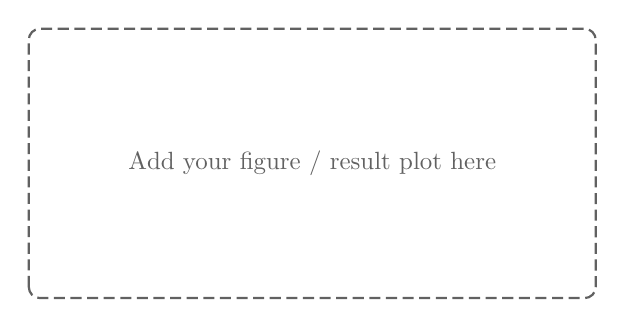
\begin{tikzpicture}[x=1cm,y=1cm]
        \draw[rounded corners, dash pattern=on 4pt off 2pt, line width=0.8pt, mygray] (0,0) rectangle (8,3.8);
        \node[mygray] at (4,1.9) {Add your figure / result plot here};
      \end{tikzpicture}%
    \end{adjustbox}
  \end{center}%
}

\newcommand{\cmark}{\textcolor{mygreen}{\ensuremath{\checkmark}}}
\newcommand{\xmark}{\textcolor{red}{\ensuremath{\times}}}

% Title page details:
\title[HW1: Generative Models]{Homework 1: Foundations of Generative Modeling\\(Lectures 0--6)}
\author{CS25 -- Large Foundation Models}
\institute[BIMSA]{Beijing Institute of Mathematical Sciences and Applications}
\date{\today}

\pgfdeclareimage[width=2cm]{logo}{../figures/logo.png}
\logo{\pgfuseimage{logo}{\vspace{-6pt}}}

\begin{document}

% ---------------- Title Page ----------------
\begin{frame}
  \titlepage
\end{frame}

\begin{frame}{Homework at a Glance}
\small
\begin{itemize}
  \item \textbf{Goal:} connect the mathematical objectives (Lectures 0--6) to working implementations and honest empirical comparisons.
  \item \textbf{You will submit:}
  \begin{itemize}
    \item \textbf{Report (PDF, 3--6 pages)}: short derivations + experiments + discussion.
    \item \textbf{Code (zip or repo link)}: training + sampling + plotting scripts/notebooks.
    \item \textbf{Reproducibility file}: README with exact run commands + environment.
  \end{itemize}
  \item \textbf{Recommended time:} 6--10 hours (depending on chosen track).
\end{itemize}
\end{frame}

\begin{frame}{Learning Objectives (Mapped to Lectures 0--6)}
\small
After this homework, you should be able to:
\begin{itemize}
  \item \textbf{Lecture 0:} summarize the ``five families'' view and trade-offs (train vs sample, likelihood vs implicit).
  \item \textbf{Lecture 1:} write down the diffusion forward process and explain score/denoising objectives.
  \item \textbf{Lecture 2:} explain flow matching as learning a velocity field and connecting it to an ODE transport.
  \item \textbf{Lecture 3:} derive the VAE ELBO and implement reparameterization.
  \item \textbf{Lecture 4:} apply change of variables and compute exact log-likelihood for a flow.
  \item \textbf{Lecture 5:} analyze GAN minimax, optimal discriminator, and practical instability.
  \item \textbf{Lecture 6:} factorize a joint distribution autoregressively and explain causal masking in Transformers.
\end{itemize}
\end{frame}

\begin{frame}{Rules \& Academic Integrity}
\small
\begin{itemize}
  \item \textbf{Work policy:} you may discuss ideas, but your derivations, code, and report must be your own.
  \item \textbf{External code:} allowed only for \emph{utility} (e.g., dataloaders, plotting). If you borrow model code, you must:
  \begin{itemize}
    \item cite it clearly (URL + what you used),
    \item explain it in your own words,
    \item and still implement \textbf{at least one core component yourself} (e.g., objective, sampling loop, masking).
  \end{itemize}
  \item \textbf{What we grade:} correctness + clarity + honest evaluation (not ``best samples on earth'').
\end{itemize}
\end{frame}

\begin{frame}{Deliverables Checklist (1/2)}
\scriptsize
\textbf{Submit these three items:} \texttt{report.pdf}, \texttt{code/} (or notebooks), \texttt{README.md}.
\vspace{0.5em}

\begin{columns}[T,onlytextwidth]
\begin{column}{0.48\textwidth}
\textbf{Report PDF}
\begin{itemize}
  \item Part A answers (A0--A6 + 2 of A7--A10)
  \item chosen Track description (what you implemented)
  \item results: figures + tables + short discussion
  \item comparison table across families (Part C)
\end{itemize}
\end{column}
\begin{column}{0.48\textwidth}
\textbf{Code}
\begin{itemize}
  \item training + sampling entrypoints
  \item evaluation/visualization code
  \item fixed random seed + hyperparameters (config or args)
  \item clear folder structure (one command to reproduce key results)
\end{itemize}
\end{column}
\end{columns}
\end{frame}

\begin{frame}{Deliverables Checklist (2/2)}
\scriptsize
\textbf{README.md must include:}
\begin{itemize}
  \item environment setup (\texttt{pip install -r requirements.txt} or equivalent)
  \item exact commands to reproduce:
  \begin{itemize}
    \item one main training run
    \item one sampling run that saves a grid/plot
    \item one evaluation/plot that generates your key figure/table
  \end{itemize}
  \item machine details (CPU/GPU) + runtime estimate (rough)
\end{itemize}

\vspace{0.4em}
\textbf{Repro rule:} if we cannot reproduce your main figure/table, you lose most reproducibility points.
\end{frame}

% ================= Part A ==================
\section{Part A: Theory (All Students)}

\begin{frame}{Part A: Theory (Make It Rigorous)}
\small
\textbf{Part A is graded like a short math assignment.} Your answers should look like clean lecture notes:
\begin{itemize}
  \item \textbf{State assumptions} (data distribution, latent variable model, differentiability, invertibility, etc.).
  \item \textbf{Show intermediate steps} for each derivation (no ``it is known that'' jumps).
  \item \textbf{Name the object you optimize} (what expectation, over which random variables).
  \item \textbf{Explain meaning} of each term (1 sentence per term is enough).
  \item \textbf{Conclude with a takeaway} (what the derivation implies for training/sampling behavior).
\end{itemize}
\vspace{0.3em}
\textbf{Write-up format:} answers A0--A10 with clear numbering (A7--A10 are the harder extensions; see slides).
\end{frame}

\begin{frame}{Part A: What Counts as a Complete Answer}
\small
For each question, we expect:
\begin{itemize}
  \item \textbf{(i) Math}: correct formula(s) with correct conditioning, distributions, and constants where needed.
  \item \textbf{(ii) A short proof/derivation}: 5--20 lines, depending on the question.
  \item \textbf{(iii) Interpretation}: 3--8 sentences connecting to the lecture (trade-offs, failure modes).
\end{itemize}
\vspace{0.4em}
\textbf{Minimum rigor rule:} if you use a known identity (e.g., Jensen, change-of-variables, KL algebra),
you must either (a) prove it briefly or (b) state it clearly and show how you apply it.
\end{frame}

\begin{frame}{Part A: Hardness Upgrade (How We Will Grade)}
\small
\begin{itemize}
  \item \textbf{Core understanding (A0--A6):} do you know the key objectives and why they work?
  \item \textbf{Deeper understanding (A7--A10):} can you connect objectives \emph{across} families and reason about failure cases?
  \item \textbf{Common deductions:}
  \begin{itemize}
    \item missing conditioning / wrong distributions,
    \item stating final results without showing steps,
    \item mixing up likelihood vs. implicit models,
    \item confusing training objective with sampling procedure.
  \end{itemize}
\end{itemize}
\end{frame}

\subsection{A0: Unifying view (Lecture 0)}

\begin{frame}{A0: The ``Five Families'' Comparison Table (Lecture 0)}
\small
\textbf{Task.} Fill in a 5-row comparison table for:
\textbf{Autoregressive}, \textbf{VAE}, \textbf{GAN}, \textbf{Normalizing Flow}, \textbf{Diffusion \emph{or} Flow Matching}.
\vspace{0.4em}

\textbf{Columns (required):}
\begin{itemize}
  \item training objective (1 line math),
  \item likelihood: exact / bound / none,
  \item sampling: one-pass / iterative / sequential,
  \item computational profile: train cost vs sample cost (qualitative),
  \item one typical failure mode (e.g., mode collapse, blurry samples, slow sampling, exposure bias, posterior collapse).
\end{itemize}
\vspace{0.4em}
\textbf{What to hand in:} one table + 3--5 sentences summarizing \emph{your} takeaway trade-off.
\end{frame}

\subsection{A1: Diffusion (Lecture 1)}

\begin{frame}{A1: Diffusion Forward Process \& Objective (Lecture 1)}
\small
\textbf{(a) Forward process.} Write a standard Gaussian noising process, e.g.
\[
x_t = \sqrt{\bar\alpha_t}\,x_0 + \sqrt{1-\bar\alpha_t}\,\epsilon,\quad \epsilon\sim \mathcal{N}(0,I),
\]
or an equivalent Markov form $q(x_t\mid x_{t-1})$.
\vspace{0.4em}

\textbf{(b) Training signal.} Choose one and write the loss precisely:
\begin{itemize}
  \item score matching ($s_\theta(x_t,t)\approx \nabla_x \log p_t(x_t)$), or
  \item $\epsilon$-prediction ($\epsilon_\theta(x_t,t)\approx \epsilon$), or
  \item $x_0$-prediction ($\hat x_{0,\theta}(x_t,t)\approx x_0$).
\end{itemize}
\vspace{0.4em}
\textbf{(c) Explanation (short).} In 3--6 sentences, explain why gradients of $\log p(x)$ (scores) avoid normalization constants in energy-based forms.
\end{frame}

\begin{frame}{A1 (Optional Challenge): Sampling and Cost}
\small
\textbf{(d) Sampling loop.} In 5--10 lines of pseudocode, write the high-level reverse sampling procedure (iterating $t=T\to 0$).
\vspace{0.4em}

\textbf{(e) Cost discussion.} Explain (2--4 sentences) why diffusion often has:
\begin{itemize}
  \item relatively stable training, but
  \item slower sampling (many steps),
\end{itemize}
and name one common acceleration idea (DDIM, fewer steps, distillation/consistency, ODE sampling, etc.).
\end{frame}

\subsection{A2: Flow matching (Lecture 2)}

\begin{frame}{A2: Flow Matching as Learning a Velocity Field (Lecture 2)}
\small
\textbf{(a) Core equation.} State the ODE transport:
\[
\frac{d x_t}{dt}=v_\theta(x_t,t),\qquad x_0\sim p_0,\ \ t\in[0,1].
\]
\textbf{(b) Continuity equation.} Write the PDE relation (strong or weak form) linking $v$ to marginals $p_t$.
\vspace{0.5em}

\textbf{(c) Regression view.} Suppose you have training pairs $(x_t,\dot x_t)$ from a chosen coupling/path.
Write the MSE loss and explain why the optimal predictor is a conditional expectation:
\[
v^\star(x,t)=\mathbb{E}[\dot x_t \mid x_t=x, t].
\]
\textbf{What to hand in:} (a)--(c) with 5--8 sentences total explanation.
\end{frame}

\subsection{A3: VAE (Lecture 3)}

\begin{frame}{A3: Derive the ELBO (Lecture 3)}
\small
\textbf{(a) Setup.} Define $p_\theta(x,z)=p_\theta(x\mid z)p(z)$ and an approximate posterior $q_\phi(z\mid x)$.
\vspace{0.4em}

\textbf{(b) Derivation.} Starting from $\log p_\theta(x)$, derive:
\[
\log p_\theta(x) \ge \mathbb{E}_{q_\phi(z\mid x)}[\log p_\theta(x\mid z)]-\mathrm{KL}\!\left(q_\phi(z\mid x)\,\Vert\,p(z)\right).
\]
\textbf{(c) Interpretation.} Label which term is reconstruction and which is regularization/prior matching.
\vspace{0.4em}

\textbf{(d) Reparameterization.} Write the reparameterization for Gaussian latents and explain (2--3 sentences) why it helps gradients.
\end{frame}

\begin{frame}{A3 (Optional Challenge): Posterior Collapse}
\small
Explain \textbf{posterior collapse} (what it is, and when it happens) in 5--8 sentences.
\vspace{0.4em}

\textbf{Must include:}
\begin{itemize}
  \item what you would observe in the KL term,
  \item why a powerful decoder can cause it,
  \item one mitigation (KL annealing, free bits, weaker decoder, $\beta$-VAE, etc.).
\end{itemize}
\end{frame}

\subsection{A4: Normalizing flows (Lecture 4)}

\begin{frame}{A4: Change of Variables and Tractable Jacobians (Lecture 4)}
\small
\textbf{(a) Formula.} For an invertible map $x=T_\theta(z)$ with $z\sim p_Z$, write:
\[
\log p_\theta(x)=\log p_Z(z)+\log\left|\det \frac{\partial T_\theta^{-1}(x)}{\partial x}\right|.
\]
\textbf{(b) Composition.} For $K$ layers, write the sum of log-determinants.
\vspace{0.5em}

\textbf{(c) Architecture reason.} Explain what structure makes determinants easy:
\begin{itemize}
  \item triangular Jacobians (autoregressive flows), or
  \item coupling layers (block triangular Jacobians),
\end{itemize}
and explicitly state what becomes ``cheap'' to compute.
\end{frame}

\subsection{A5: GANs (Lecture 5)}

\begin{frame}{A5: GAN Minimax and Optimal Discriminator (Lecture 5)}
\small
\textbf{(a) Objective.} Write the minimax GAN objective:
\[
\min_G \max_D\ \mathbb{E}_{x\sim p_{\text{data}}}[\log D(x)]+\mathbb{E}_{z\sim p_z}[\log(1-D(G(z)))].
\]
\textbf{(b) Optimal $D$.} For fixed $G$, derive:
\[
D_G^*(x)=\frac{p_{\text{data}}(x)}{p_{\text{data}}(x)+p_g(x)}.
\]
\textbf{(c) Divergence link.} Substitute $D^*_G$ and show the Jensen--Shannon divergence form (you may skip constant terms if you state them).
\vspace{0.4em}

\textbf{What to hand in:} derivation steps (not just the final line) + 3--6 sentences on what this says about convergence.
\end{frame}

\begin{frame}{A5 (Optional Challenge): Training Instability}
\small
Give \textbf{two} reasons GAN training is unstable in practice (e.g., non-convex game dynamics, discriminator too strong/weak, vanishing gradients, support mismatch).
\vspace{0.4em}

\textbf{Then:} name \textbf{one} stabilization idea and briefly justify it:
\begin{itemize}
  \item non-saturating loss, WGAN, gradient penalty, spectral norm, EMA, etc.
\end{itemize}
\end{frame}

\subsection{A6: Autoregressive models \& Transformers (Lecture 6)}

\begin{frame}{A6: Autoregressive Factorization (Lecture 6)}
\small
\textbf{(a) Factorization.} For a sequence $x_{1:T}$, write:
\[
p(x_{1:T})=\prod_{t=1}^T p(x_t\mid x_{<t})
\quad \Longleftrightarrow \quad
\log p(x_{1:T})=\sum_{t=1}^T \log p(x_t\mid x_{<t}).
\]
\textbf{(b) MLE loss.} Write the negative log-likelihood (cross-entropy) training objective for a dataset.
\vspace{0.5em}

\textbf{(c) Sampling.} Explain (3--5 sentences) why sampling is sequential and how this differs from one-pass flows.
\end{frame}

\begin{frame}{A6: Causal Masking in Self-Attention (Lecture 6)}
\small
\textbf{(a) Attention.} Write the (scaled) dot-product attention:
\[
\mathrm{Attn}(Q,K,V)=\mathrm{softmax}\!\left(\frac{QK^\top}{\sqrt{d}}\right)V
\]
(you may omit multi-head details).
\vspace{0.4em}

\textbf{(b) Mask.} Define a causal mask $M$ that prevents attending to future tokens (state what entries are $-\infty$ vs $0$).
\vspace{0.4em}

\textbf{(c) Reasoning.} In 4--8 sentences, explain how masking enforces dependence only on $x_{<t}$ and connects to the AR factorization in A6(a).
\end{frame}

% ================= Harder extensions ==================
\subsection{A7--A10: Harder Theory Extensions (Required)}

\begin{frame}{A7--A10: Harder Theory Extensions (Required)}
\small
\textbf{These are the harder questions.} Answer \textbf{at least 2 out of A7--A10} (you may answer all for bonus).
\vspace{0.4em}

\textbf{Why:} these force you to connect the lectures, not just restate definitions.
\vspace{0.4em}

\textbf{What to hand in:} for each chosen question, include (i) derivation/proof sketch, (ii) interpretation, (iii) one concrete implication for practice.
\end{frame}

\subsection{A7: Diffusion objective equivalences}

\begin{frame}{A7: Diffusion --- Relating $\epsilon$-Prediction to Score (Lecture 1)}
\small
Assume the standard Gaussian corruption
\[
x_t = \sqrt{\bar\alpha_t}\,x_0 + \sqrt{1-\bar\alpha_t}\,\epsilon,\qquad \epsilon\sim\mathcal{N}(0,I).
\]
\textbf{(a)} Derive the conditional score $\nabla_{x_t}\log q(x_t\mid x_0)$ in closed form.
\vspace{0.3em}

\textbf{(b)} Show the algebraic relationship between the score and the noise:
\[
\nabla_{x_t}\log q(x_t\mid x_0) = -\frac{1}{\sqrt{1-\bar\alpha_t}}\ \epsilon.
\]
\textbf{(c)} Use (b) to explain (with equations) why training an $\epsilon_\theta(x_t,t)$ network can be viewed as a form of score learning (up to scaling).
\vspace{0.3em}

\textbf{(d) Interpretation:} in 5--8 sentences, explain what this says about ``why $\epsilon$-prediction works'' and what changes if the noise is not Gaussian.
\end{frame}

\subsection{A8: Flow matching / CNF connection}

\begin{frame}{A8: Flow Matching --- Continuity Eq. \& Log-Density Dynamics (Lectures 2 \& 4)}
\small
Let $x_t$ follow the ODE $\dot x_t=v(x_t,t)$ and let $p_t$ be the density of $x_t$.
\textbf{(a)} Starting from the continuity equation
\[
\partial_t p_t(x)+\nabla\cdot(p_t(x)v(x,t))=0,
\]
derive the \textbf{log-density} evolution along trajectories:
\[
\frac{d}{dt}\log p_t(x_t) = -\,\nabla\cdot v(x_t,t).
\]
\textbf{(b)} Explain why (a) is the key identity behind continuous normalizing flows (CNFs).
\vspace{0.3em}

\textbf{(c)} In 5--8 sentences, compare the training signal in flow matching (regress a velocity) vs. in diffusion (learn a score) and discuss one scenario where one signal is easier to obtain than the other.
\end{frame}

\subsection{A9: ELBO gaps and posterior collapse}

\begin{frame}{A9: VAE --- ELBO Gap and What KL Is Really Measuring (Lecture 3)}
\small
Let $p_\theta(x,z)=p_\theta(x\mid z)p(z)$ and $q_\phi(z\mid x)$.
\textbf{(a)} Prove the ``ELBO gap'' identity:
\[
\log p_\theta(x)-\mathrm{ELBO}(x)
=\mathrm{KL}\!\left(q_\phi(z\mid x)\,\Vert\,p_\theta(z\mid x)\right)\ge 0.
\]
\textbf{(b)} Expand the dataset-averaged KL term
$\mathbb{E}_{p_{\text{data}}(x)}\mathrm{KL}(q_\phi(z\mid x)\Vert p(z))$
into a sum involving \textbf{mutual information} $I_q(x;z)$ and a marginal KL $\mathrm{KL}(q_\phi(z)\Vert p(z))$ (state your definition of $q_\phi(z)$).
\vspace{0.3em}

\textbf{(c) Interpretation:} explain how (b) clarifies posterior collapse and why it is linked to the decoder strength.
\end{frame}

\subsection{A10: GAN gradients and support mismatch}

\begin{frame}{A10: GAN --- Why Gradients Can Vanish (Lecture 5)}
\small
Consider the original GAN with optimal discriminator $D^*_G(x)$.
\textbf{(a)} Assume $p_{\text{data}}$ and $p_g$ have (approximately) disjoint support early in training.
Use $D^*_G(x)=\frac{p_{\text{data}}(x)}{p_{\text{data}}(x)+p_g(x)}$ to argue what values $D^*_G$ takes on real vs fake regions.
\vspace{0.3em}

\textbf{(b)} Using (a), explain (with a short derivative argument) why the generator gradient can become very small for the minimax loss.
\vspace{0.3em}

\textbf{(c)} Propose one fix and justify it mathematically at a high level:
\begin{itemize}
  \item non-saturating loss, or
  \item Wasserstein GAN idea (name the key theorem/constraint: 1-Lipschitz critic).
\end{itemize}
\end{frame}

% ================= Part B ==================
\section{Part B: Implementation (Choose One Track)}

\begin{frame}{Part B: Choose One Track}
\small
Pick \textbf{exactly one} implementation track (B1/B2/B3). Each track asks you to implement and evaluate \textbf{at least two model families} from Lectures 1--6.
\vspace{0.75em}

\begin{tabular}{@{}p{0.18\linewidth}p{0.76\linewidth}@{}}
\toprule
\textbf{Track} & \textbf{Summary} \\
\midrule
B1: Toy 2D & Implement \textbf{Flow} (Lecture 4) \emph{and} \textbf{GAN} (Lecture 5) on a 2D mixture (fast, great for debugging). \\
B2: MNIST & Implement \textbf{VAE} (Lecture 3) \emph{and} one of: \textbf{Diffusion} (Lecture 1) or \textbf{GAN} (Lecture 5). \\
B3: Tiny text & Implement a \textbf{Transformer LM} (Lecture 6) \emph{and} a baseline (e.g., bigram/MLP autoregressive) and compare. \\
\bottomrule
\end{tabular}
\end{frame}

\begin{frame}{Common Requirements for All Tracks}
\small
\begin{itemize}
  \item \textbf{Reproducibility:} fix a random seed; log hyperparameters.
  \item \textbf{Training curve:} show at least one meaningful curve (loss, NLL, reconstruction, discriminator metrics).
  \item \textbf{Sampling:} generate and visualize at least 64 samples per model.
  \item \textbf{Comparison table:} include a table comparing the two chosen families on:
  \begin{itemize}
    \item training time, sampling time, stability, and qualitative sample diversity.
  \end{itemize}
\end{itemize}
\end{frame}

\subsection{Track B1: Toy 2D (Flow + GAN)}

\begin{frame}{Track B1: Dataset \& Target}
\small
\textbf{Dataset:} 2D mixture of Gaussians (e.g., 8 Gaussians in a circle) or ``two moons''.
\begin{itemize}
  \item Implement a \textbf{normalizing flow} (Lecture 4) that allows exact log-likelihood.
  \item Implement a \textbf{GAN} (Lecture 5) and compare coverage vs mode collapse.
\end{itemize}
\vspace{0.4em}
\textbf{Plots to include:}
\begin{itemize}
  \item scatter of real data vs generated samples,
  \item density heatmap for the flow (optional but recommended),
  \item training curves (NLL for flow; discriminator/generator losses for GAN).
\end{itemize}
\end{frame}

\begin{frame}{Track B1: Minimal Model Specs (Suggested)}
\small
\begin{itemize}
  \item \textbf{Flow:} 6--12 coupling layers; MLP conditioner; base $\mathcal{N}(0,I)$.
  \item \textbf{GAN:} MLP generator + MLP discriminator; use non-saturating loss; consider gradient penalty as a stability add-on (optional).
  \item \textbf{Evaluation:} for GAN, report a simple \emph{coverage metric} (e.g., cluster assignment proportions) + show multiple random seeds.
\end{itemize}
\end{frame}

\subsection{Track B2: MNIST (VAE + Diffusion or GAN)}

\begin{frame}{Track B2: Dataset \& Target}
\small
\textbf{Dataset:} MNIST (28$\times$28 grayscale) via \texttt{torchvision.datasets.MNIST}.
\begin{itemize}
  \item Implement a \textbf{VAE} (Lecture 3) with convolutional encoder/decoder (or MLP if you prefer).
  \item Implement \textbf{either}:
  \begin{itemize}
    \item a small \textbf{diffusion model} (Lecture 1) with a tiny U-Net, \emph{or}
    \item a simple \textbf{DCGAN-style} model (Lecture 5).
  \end{itemize}
\end{itemize}
\vspace{0.4em}
\textbf{Must include:} sample grids + a short note on typical failure mode (blurry VAE vs instability or slow sampling).
\end{frame}

\begin{frame}{Track B2: Minimal Model Specs (Suggested)}
\small
\begin{itemize}
  \item \textbf{VAE:} latent dim 16--64; report reconstruction term and KL term separately.
  \item \textbf{Diffusion:} 50--200 steps (small); noise schedule of your choice; train $\epsilon_\theta(x_t,t)$.
  \item \textbf{GAN:} monitor mode collapse (visualize samples over time); try label smoothing or gradient penalty (optional).
\end{itemize}
\end{frame}

\subsection{Track B3: Tiny Text (Transformer + Baseline)}

\begin{frame}{Track B3: Dataset \& Target}
\small
\textbf{Dataset:} a small text corpus (you choose; keep it under $\sim$5MB).
\begin{itemize}
  \item Implement an \textbf{autoregressive Transformer} (Lecture 6) with causal masking.
  \item Implement a \textbf{baseline} autoregressive model (bigram, n-gram, or MLP with a fixed context window).
\end{itemize}
\vspace{0.4em}
\textbf{Must include:}
\begin{itemize}
  \item training curves (NLL/perplexity),
  \item samples at different temperatures,
  \item short explanation of why masking is needed (connect to factorization).
\end{itemize}
\end{frame}

\begin{frame}{Track B3: Minimal Model Specs (Suggested)}
\small
\begin{itemize}
  \item \textbf{Tokenizer:} character-level is fine (fast + simple).
  \item \textbf{Transformer:} 2--4 layers, 4 heads, d\_model 128--256.
  \item \textbf{Evaluation:} report validation NLL/perplexity; show 3 sample generations with different seeds.
\end{itemize}
\end{frame}

% ================= Part C ==================
\section{Part C: Comparison \& Discussion}

\begin{frame}{Part C: Comparison Table (Required)}
\small
Include a table comparing your two implemented families. Suggested columns:
\begin{itemize}
  \item \textbf{Objective} (NLL / ELBO / minimax / denoising / regression).
  \item \textbf{Likelihood?} exact / bound / none.
  \item \textbf{Sampling} one pass / iterative ODE-SDE / autoregressive.
  \item \textbf{Stability issues} and what you observed.
  \item \textbf{Best use-case} based on your results and Lectures 0--6.
\end{itemize}
\end{frame}

\begin{frame}{Part C: What We Look For in the Discussion}
\small
\begin{itemize}
  \item \textbf{Honesty}: show failures; explain them using lecture concepts (mode collapse, posterior collapse, slow sampling, exposure bias, etc.).
  \item \textbf{Ablation (small)}: change one hyperparameter and report the effect (e.g., latent dim, number of flow layers, diffusion steps, learning rate).
  \item \textbf{Trade-offs}: connect your measurements to the Lecture 0 taxonomy.
\end{itemize}
\end{frame}

% ================= Logistics ==================
\section{Logistics}

\begin{frame}{Submission Format}
\small
\begin{itemize}
  \item Submit a single \textbf{zip} (or a repo link) containing:
  \begin{itemize}
    \item \texttt{report.pdf}
    \item \texttt{code/} (or notebooks)
    \item \texttt{README.md} with exact commands
    \item \texttt{requirements.txt} or environment spec
  \end{itemize}
  \item \textbf{Naming:} \texttt{CS25\_HW1\_<YourName>.zip}
  \item \textbf{Late policy:} fill in according to course policy.
\end{itemize}
\end{frame}

\begin{frame}{Grading Rubric}
\small
\begin{tabular}{@{}p{0.25\linewidth}p{0.65\linewidth}@{}}
\toprule
\textbf{Category} & \textbf{What we grade} \\
\midrule
Theory (35\%) & correctness, clean derivations, correct connections to Lectures 0--6 \\
Implementation (35\%) & correct training + sampling, sensible code structure, reproducibility \\
Experiments (20\%) & plots, samples, at least one ablation, honest comparison \\
Communication (10\%) & report clarity, tables/figures labeled, limitations stated \\
\bottomrule
\end{tabular}
\end{frame}

\begin{frame}{FAQ}
\small
\begin{itemize}
  \item \textbf{Do I need a GPU?} No. B1 and B3 run fine on CPU; B2 is easier with a GPU but can be scaled down.
  \item \textbf{Can I pick different model pairs?} Ask first; we want coverage of Lectures 1--6.
  \item \textbf{How much code is expected?} Minimal and correct beats large and brittle.
  \item \textbf{Can I use existing libraries (e.g., diffusers)?} For this HW, prefer implementing core logic yourself.
\end{itemize}
\end{frame}

\begin{frame}{Reminder: Connect Back to the Course}
\small
\textbf{Your report should explicitly reference lecture concepts} when interpreting results:
\begin{itemize}
  \item Likelihood vs implicit modeling (Lecture 0)
  \item Scores and denoising (Lecture 1)
  \item ODE transport and conditional expectation (Lecture 2)
  \item ELBO terms and posterior collapse (Lecture 3)
  \item Jacobians and tractable determinants (Lecture 4)
  \item Minimax dynamics and mode collapse (Lecture 5)
  \item Factorization and masking (Lecture 6)
\end{itemize}
\end{frame}

\end{document}


